%%%%%%%%%%%%%%%%%%%%%%%%%%%%%%%%%%%%%%%%%
% Jacobs Landscape Poster
% LaTeX Template
% Version 1.0 (29/03/13)
%
% Created by:
% Computational Physics and Biophysics Group, Jacobs University
% https://teamwork.jacobs-university.de:8443/confluence/display/CoPandBiG/LaTeX+Poster
% 
% Further modified by:
% Nathaniel Johnston (nathaniel@njohnston.ca)
%
% This template has been downloaded from:
% http://www.LaTeXTemplates.com
%
% License:
% CC BY-NC-SA 3.0 (http://creativecommons.org/licenses/by-nc-sa/3.0/)
%
%%%%%%%%%%%%%%%%%%%%%%%%%%%%%%%%%%%%%%%%%
%---------------------------------------------------------------------
%   CONFIGURACION GENERAL
%---------------------------------------------------------------------
\documentclass[final]{beamer}
\usepackage[scale=1.24]{beamerposter} % Use the beamerposter package for laying out the poster
\usetheme{confposter} % Use the confposter theme supplied with this template

%Configurando secciones ['Cuadros de texto' pa los cuates] hay de dos tipos
%1) El puro texto (Sin un marco)
\setbeamercolor{block title}{fg=purple,bg=white} % Bloques (Sin cuadro) - Titulo
\setbeamercolor{block body}{fg=black,bg=white} % Bloques - cuerpo
%2) El texto con marco
\setbeamercolor{block alerted title}{fg=white,bg=dblue!70} % Cuadros - Titulo
\setbeamercolor{block alerted body}{fg=black,bg=dblue!10} % Cuadros - Cuerpo

%-----------------------------------------------------------
% MEDIDAS DEL POSTER
%----------------------------------------------------------
% To set effective sepwid, onecolwid and twocolwid values, first choose how many columns you want and how much separation you want between columns
% In this template, the separation width chosen is 0.024 of the paper width and a 4-column layout
% onecolwid should therefore be (1-(# of columns+1)*sepwid)/# of columns e.g. (1-(4+1)*0.024)/4 = 0.22
% Set twocolwid to be (2*onecolwid)+sepwid = 0.464
% Set threecolwid to be (3*onecolwid)+2*sepwid = 0.708

\newlength{\sepwid}
\newlength{\onecolwid}
\newlength{\twocolwid}
\newlength{\threecolwid}
\setlength{\paperwidth}{62.99in} % Width 150 cm  [Max 96in - 244 cm]
\setlength{\paperheight}{43.307in} % Heighth 120.22 [Max 48 - 121 m]
\setlength{\sepwid}{0.01\paperwidth} % Separation width (white space) between columns
\setlength{\onecolwid}{0.24\paperwidth} % Width of one column
\setlength{\twocolwid}{0.464\paperwidth} % Width of two columns
\setlength{\threecolwid}{0.708\paperwidth} % Width of three columns
\setlength{\topmargin}{0in} % Reduce the top margin size
%-----------------------------------------------------------
% PAQUETES PA' HACER EL POSTER
%-------------------------------------------

\usepackage{graphicx}  % Required for including images
\usepackage[utf8]{inputenc}
\usepackage[portuges, brazil]{babel}   
\usepackage{booktabs} % Top and bottom rules for tables

%----------------------------------------------------------------------------------------
%   TITULO & LOGOS
%----------------------------------------------------------------------------------------

\title{The Mirror Effect within Perception: Not another Recognition Memory Study} % Poster title
\author{Adriana F. Chávez De la Peña} % Author(s)
\institute{National Autonomous University of Mexico (UNAM); Faculty of Psychology\\ Lab 25;  PAPIIT IN307214 - PAPIME PE310016} % Institution(s)

\begin{document}
\addtobeamertemplate{block end}{}{\vspace*{1.5ex}} % White space under blocks
\addtobeamertemplate{block alerted end}{}{\vspace*{1.5ex}} % White space under highlighted (alert) blocks
\setlength{\belowcaptionskip}{1ex} % White space under figures
\setlength\belowdisplayshortskip{1ex} % White space under equations
\begin{frame}[t] % The whole poster is enclosed in one beamer frame
\begin{tikzpicture}[remember picture,overlay]
\node[anchor=north west] at ([shift={(5cm,-1cm)}]current page.north west)
    {
\includegraphics[width=10cm]{Figures/UNAMiwi.jpg}};
\node[anchor=north east] at ([shift={(-5cm,-1cm)}]current page.north east)
    {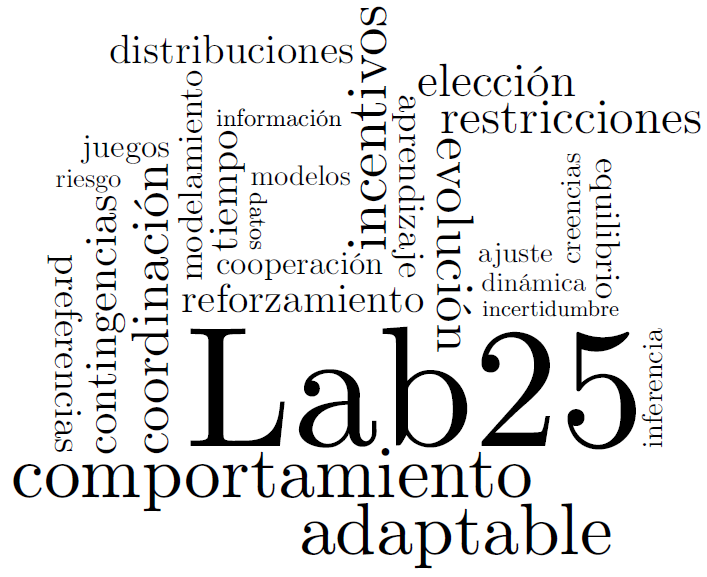
\includegraphics[width=12cm]{Figures/Lab25.png}};
\end{tikzpicture}

%-----------------------------------------------------------------------------------------
%----------------------------------------------------------------------------------------
%   PRIMERA COLUMNA
%----------------------------------------------------------------------------------------
%   INTRODUCCION
%-------------------------------|||

\begin{columns}[t] % The whole poster consists of three major columns, the second of which is split into two columns twice - the [t] option aligns each column's content to the top
\begin{column}{\sepwid}\end{column} % Empty spacer column
\begin{column}{\onecolwid} % The first column


\setbeamercolor{block alerted title}{fg=white,bg=jblue}
\setbeamercolor{block alerted body}{fg=black,bg=jblue!10}
\begin{alertblock}{Introduction: A memory phenomenon?}

Signal Detection Theory has been applied to Recognition Memory studies to describe subjects’ ability to discriminate between stimuli that have been presented before from a new set of stimuli. When comparing subjects' performance between two classes of stimuli, one being more easily recognized (A) than the other (B), the response patterns obtained show that the difference in their discriminability is reflected in the identification of both target and lure stimuli, a phenomenom now known as the Mirror Effect (Glanzer et al., 1993).


\begin{figure}
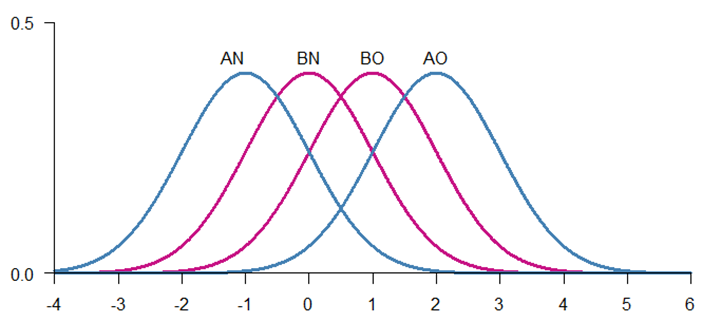
\includegraphics[width=0.5\linewidth]{Figures/MirrorEffect.png}
\end{figure}

Evidence in favor of the Mirror Effect has been reported in Recognition Memory across different SDT-alike procedures. In typical Yes/No tasks, it appears as:

\begin{equation}
FA(A) < FA(B) < Hits(B) < Hits(A)
\label{eqn:Rates}
\end{equation}

In Confidence Rating procedures, it has been found that:

\begin{equation}
R(AN) < R(BN) < R(BS) < R(AS)
\label{eqn:Confidence}
\end{equation}

However, the Mirror Effect has only been studied within Recognition Memory and so, most theories and models proposed to explain it tend to do it in terms of high-level processes engaged in the study phase. The main goal of the present study was to explore the existence of the Mirror Effect in a decision task that only involves perception.
\end{alertblock}


%------------------------------------------------------------------------------------------
% METODO & PROCEDIMIENTO
%-----------------------------------------|||||

\setbeamercolor{block alerted title}{fg=white,bg=jblue} % Titulo del Cuadro
\setbeamercolor{block alerted body}{fg=black,bg=white} % Cuerpo / Contenido del cuadro
\begin{alertblock}{Method: A perceptual task}

\textbf{Ebbinghaus illusion: Two levels of perceptual discriminability} (Massaro \& Anderson  1971).

\begin{itemize}
\item High accuracy (A): 2 or 3 surrounding circles.
\item Low accuracy (B): 7 or 8 surrounding circles.
\end{itemize}

$\quad$
\setbeamercolor{item}{fg=Purple}
\setbeamercolor{item projected}{fg=white,bg=Purple}
\begin{enumerate}
\item \textbf{Detection Task:} Are the central circles the same size?
\begin{tabular}{ccc}
$\qquad$ 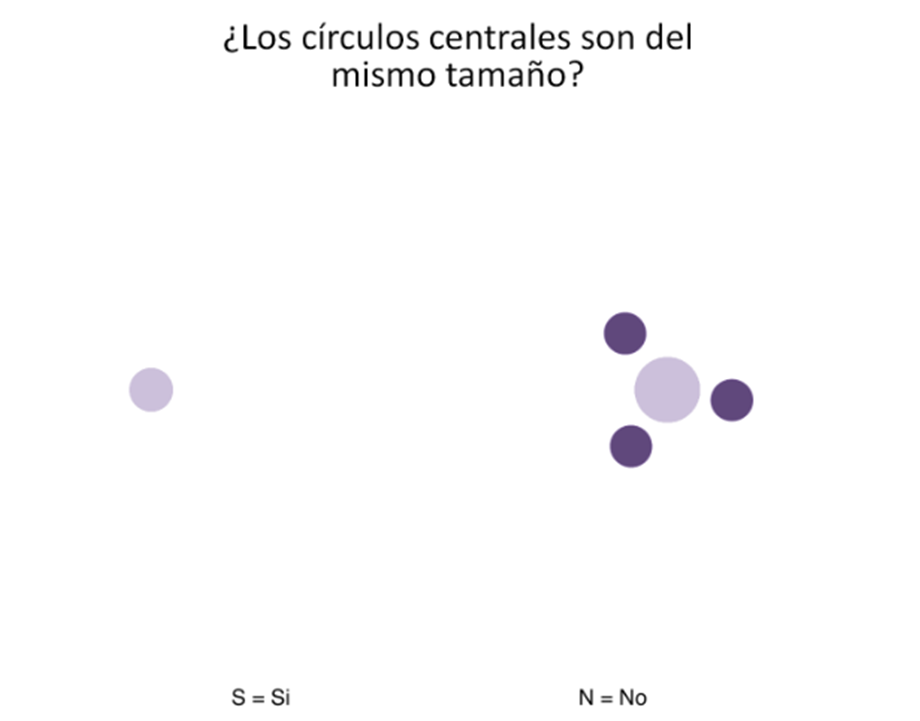
\includegraphics[width=0.35\linewidth]{Figures/MainTask.png} & \hfill & $\qquad$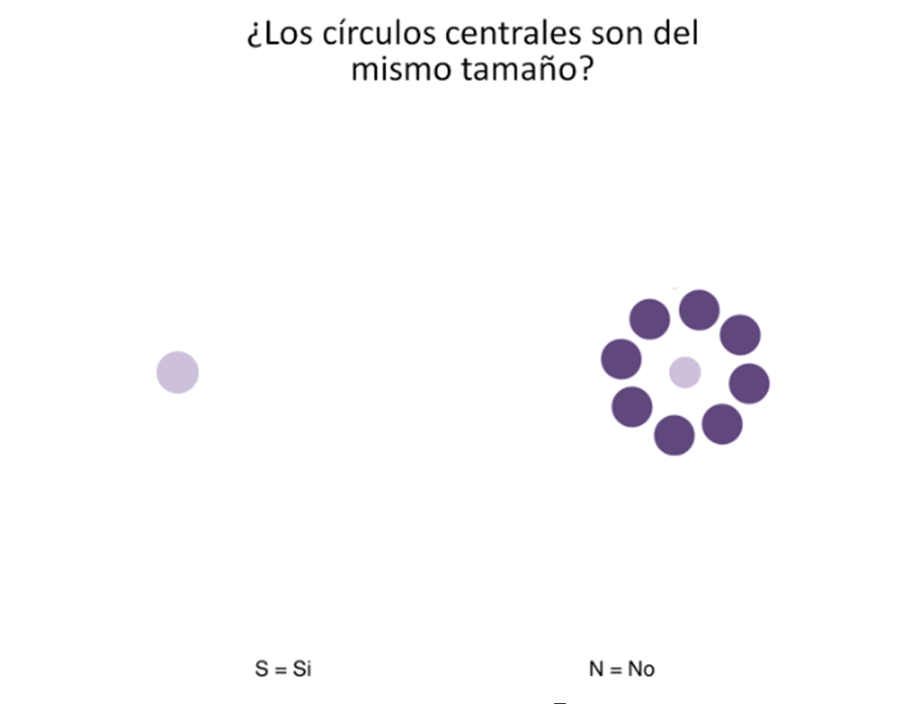
\includegraphics[width=0.35\linewidth]{Figures/MainTask2.png}
\end{tabular}
\item \textbf{Confidence Rating}
\end{enumerate}
$\qquad$

\textbf{Two experiments:} 

\begin{itemize}
\item Experiment 1: Just the right circle was an Ebbinghaus illusion.
\item Experiment 2: Both circles were constructed as Ebbinghaus illusions.
\end{itemize}

$\qquad$

\textbf{Technical details:} 

\begin{itemize}
\item 640 trials (total)
%	\item 340 - A condition |  340 - B condition
%		\item 160 - Noise | 160 - Signal
%\item 40 different stimuli, (10 repetitions, at least)
%	\item 16 different noise stimuli per condition
%	\item 4 different signal stimuli per condition
\item 1.5 s exposure
\end{itemize}
\end{alertblock}

%-----------------------------------------------------------------------------------------
% FIN PRIMERA COLUMNA
%-----------------------------------------------------------------------------------------

\end{column} % End of the first column

\begin{column}{\sepwid}\end{column} % Empty spacer column

\begin{column}{\twocolwid} % Begin a column which is two columns wide (column 2)


%----------------------------------------------------------------------------------------
% RESULTADOS GENERALES
%----------------------------------------------------------------------------------------

\setbeamercolor{block alerted title}{fg=white,bg=jblue}
\setbeamercolor{block alerted body}{fg=black,bg=jblue!10}
\begin{alertblock}{What did we find? (General Results)}

We had 20 and 21 participants on Experiments 1 and 2 respectively. In both cases, we found evidence for the Mirror Effect in at least 85\% of the participants. In Experiment 1, we had 17 cases showing the Mirror Effect pattern within the hit and false alarm rates and 18 in terms of Confidence Ratings. In Experiment 2 we had 19 participants showing the Mirror Effect in both patterns of response. All these proportions were statistically significant when we apply a simple Binomial Test (p=0.0025 and p=0.0004, for Experiment 1, and p=0.0002 for Experiment 2).

\end{alertblock} 

%----------------------------------------------------------------------------------------
%   ANALISIS POR REPLICA 
%-------------------------------||||||||
\setlength{\onecolwid}{0.24\paperwidth}
\begin{columns}[t,totalwidth=\twocolwid] % Split up the two columns wide column
\begin{column}{\onecolwid}\vspace{-.6in} % The first column within column 2 (column 2.1)


\setbeamercolor{block alerted title}{fg=white,bg=jblue} % Change the alert block title colors
\setbeamercolor{block alerted body}{fg=black,bg=white} % Change the alert block body colors
\begin{alertblock}{Data}


% set colors for itemize/enumerate
\setbeamercolor{item}{fg=Violet}
\setbeamercolor{item projected}{fg=white,bg=Violet}
\begin{itemize}
\item Are there changes in participants' performance across time?

\begin{center}
\begin{tabular}{ccc}
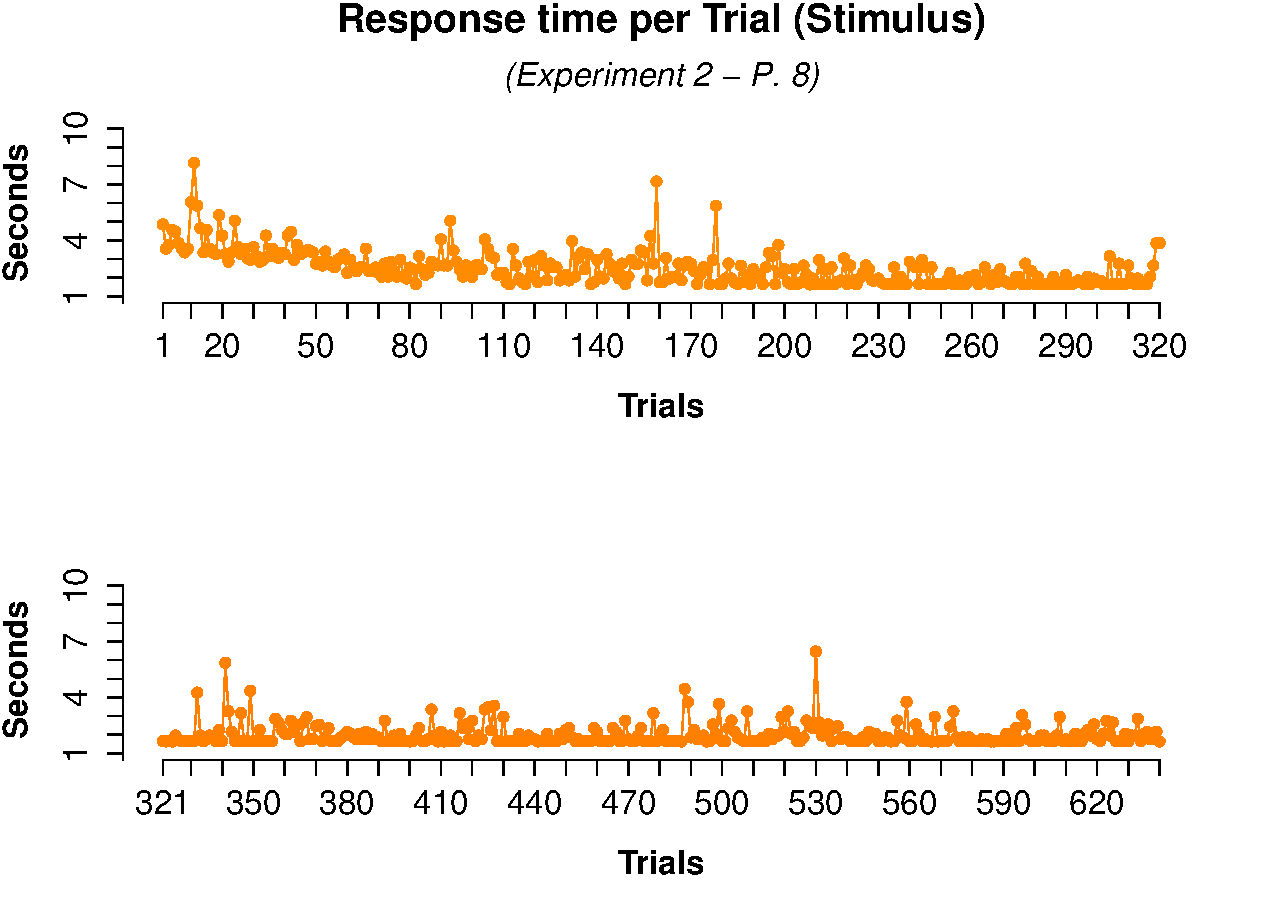
\includegraphics[width=0.49\linewidth]{Figures/4_RT_St.pdf} & \hfill & 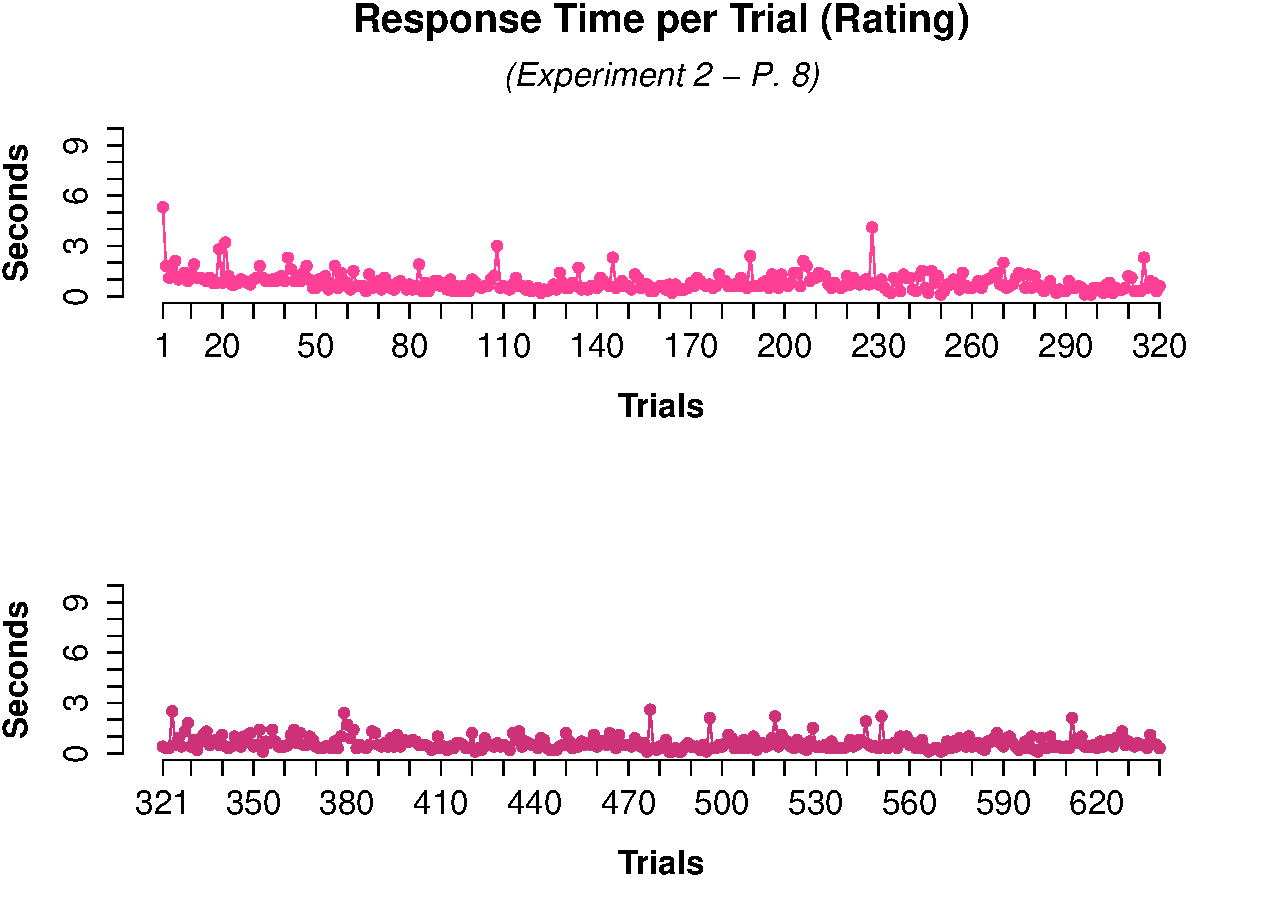
\includegraphics[width=0.49\linewidth]{Figures/4_RT_CR.pdf}
\end{tabular}
\end{center}


\begin{center}
\begin{tabular}{ccc}
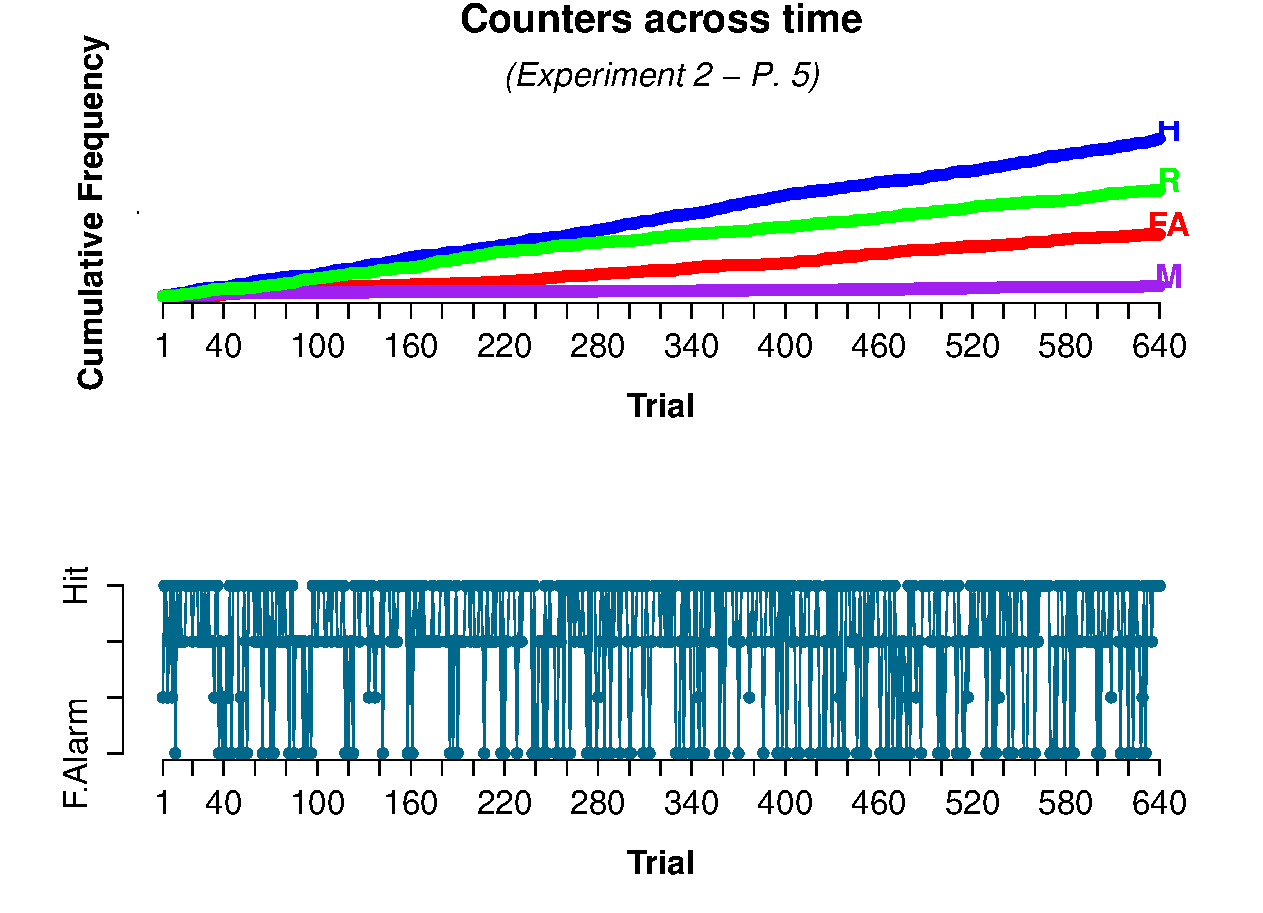
\includegraphics[width=0.49\linewidth]{Figures/2_Counters.pdf} & \hfill & 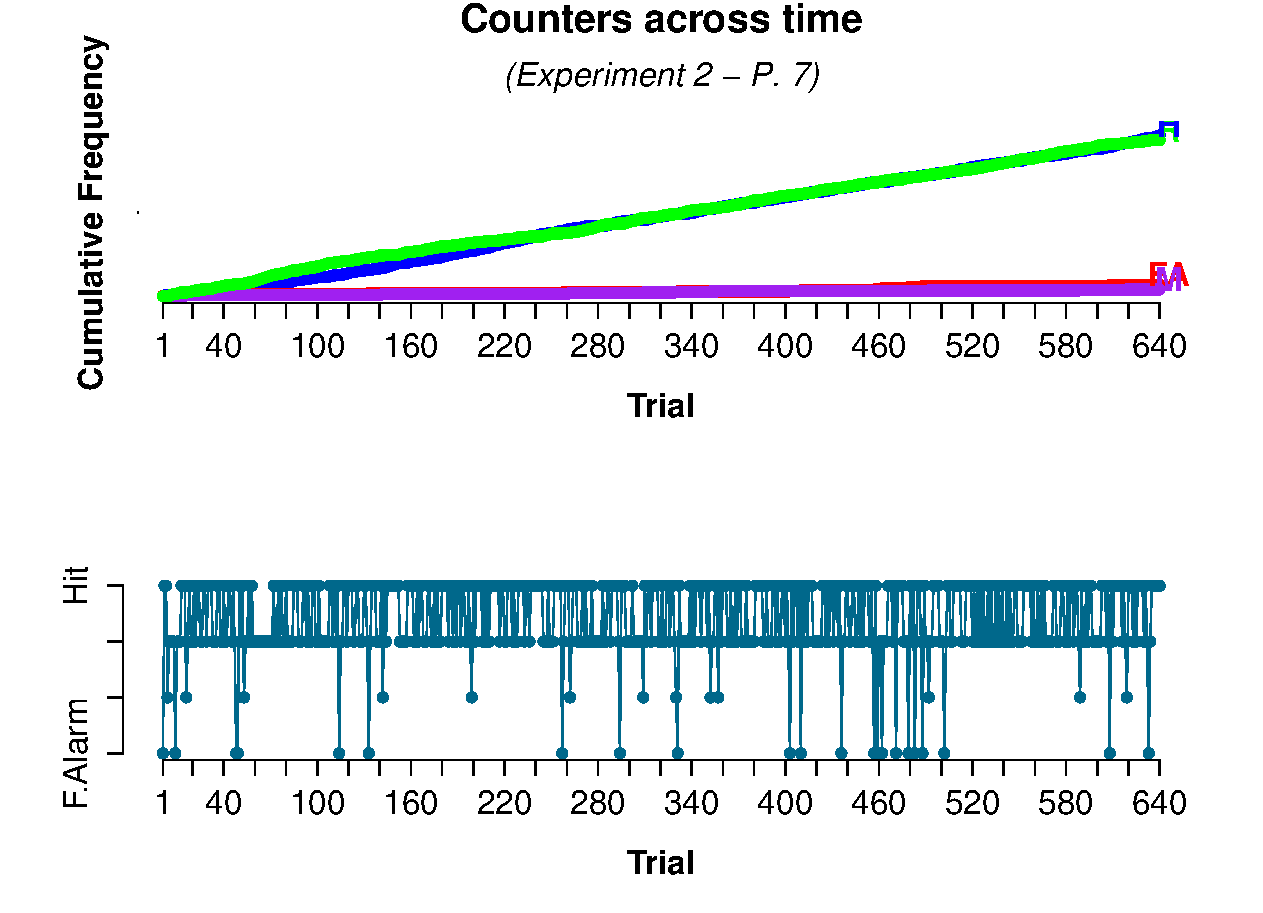
\includegraphics[width=0.49\linewidth]{Figures/2_Counters_.pdf}
\end{tabular}
\end{center}


\item Are participants actually paying attention?

\begin{center}
\begin{tabular}{ccc}
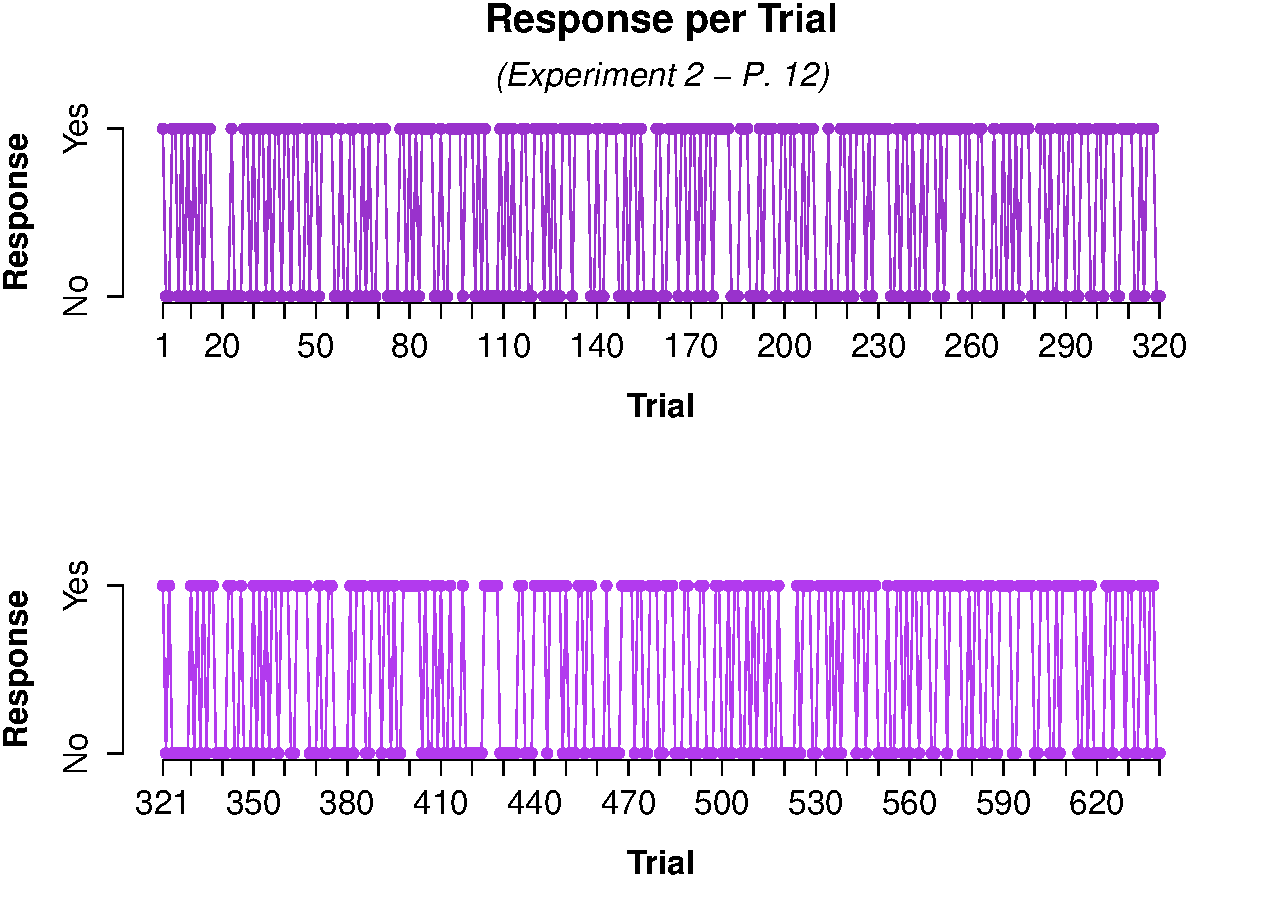
\includegraphics[width=0.48\linewidth]{Figures/5_CR.pdf} & \hfill & 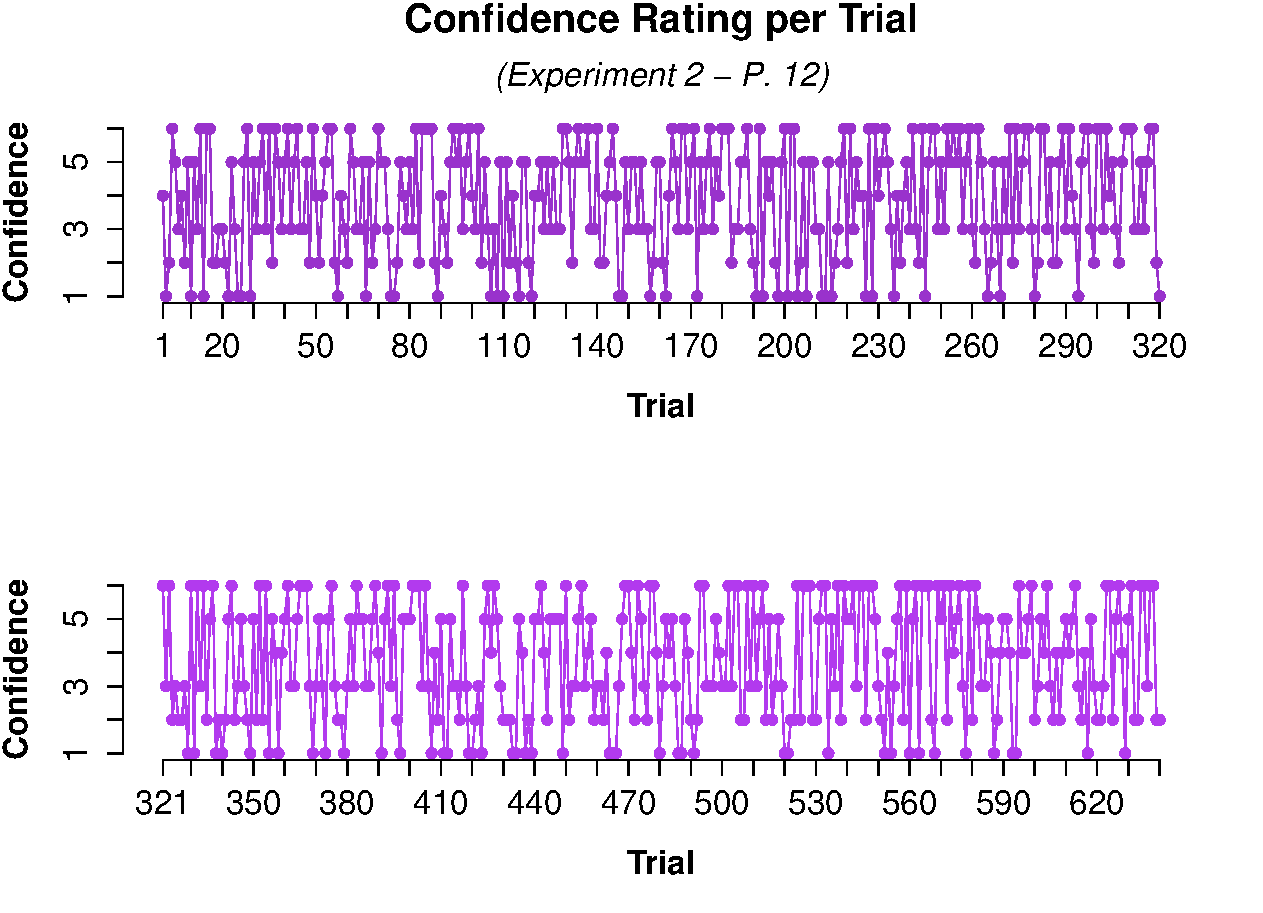
\includegraphics[width=0.48\linewidth]{Figures/6_ChoicePer.pdf}
\end{tabular}
\end{center}


\item Are the variables involved within stimuli affecting participants' responses?

\begin{center}
\begin{tabular}{ccc}
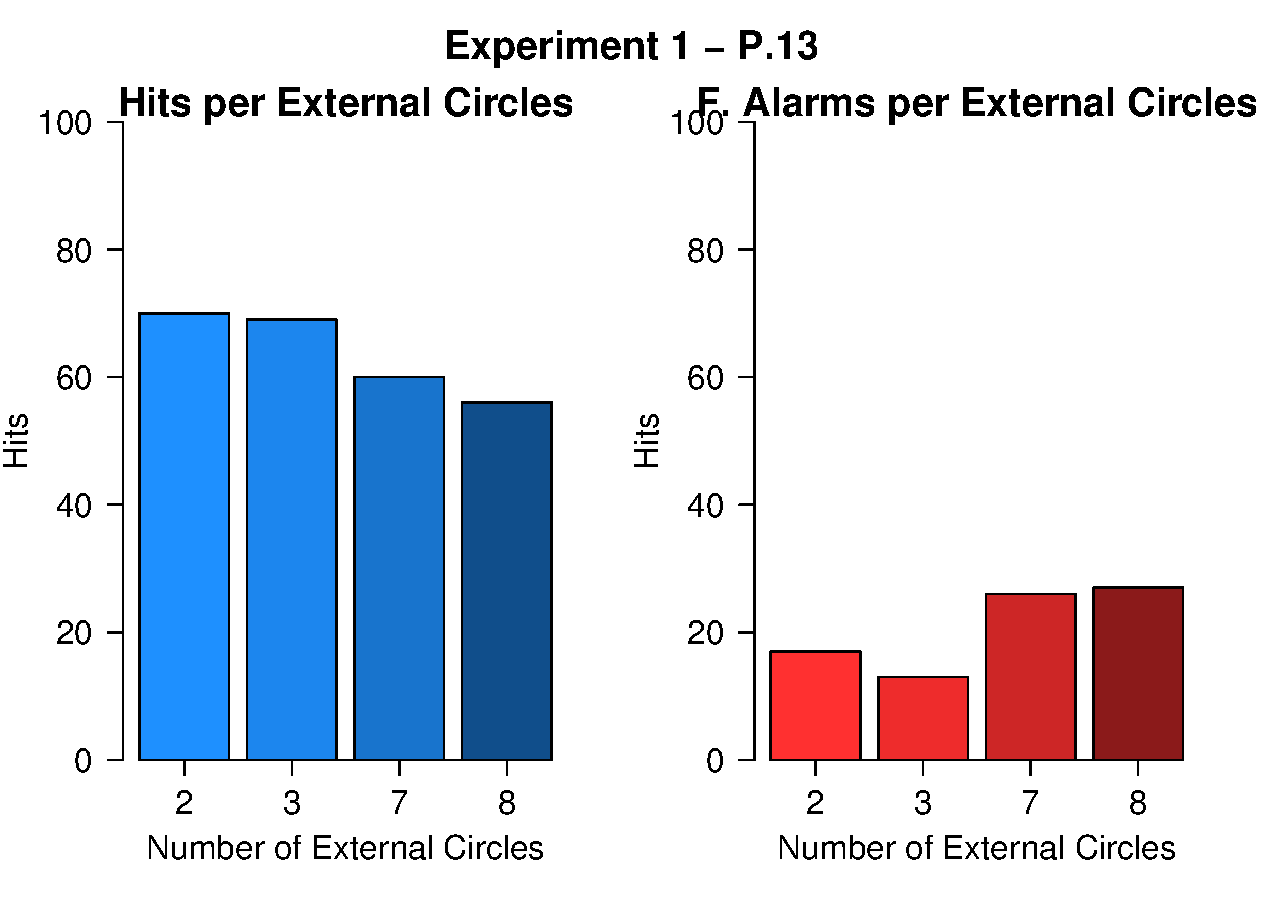
\includegraphics[width=0.45\linewidth]{Figures/7_ExternalC.pdf} 
\end{tabular}
\end{center}


\begin{center}
\begin{tabular}{ccc}
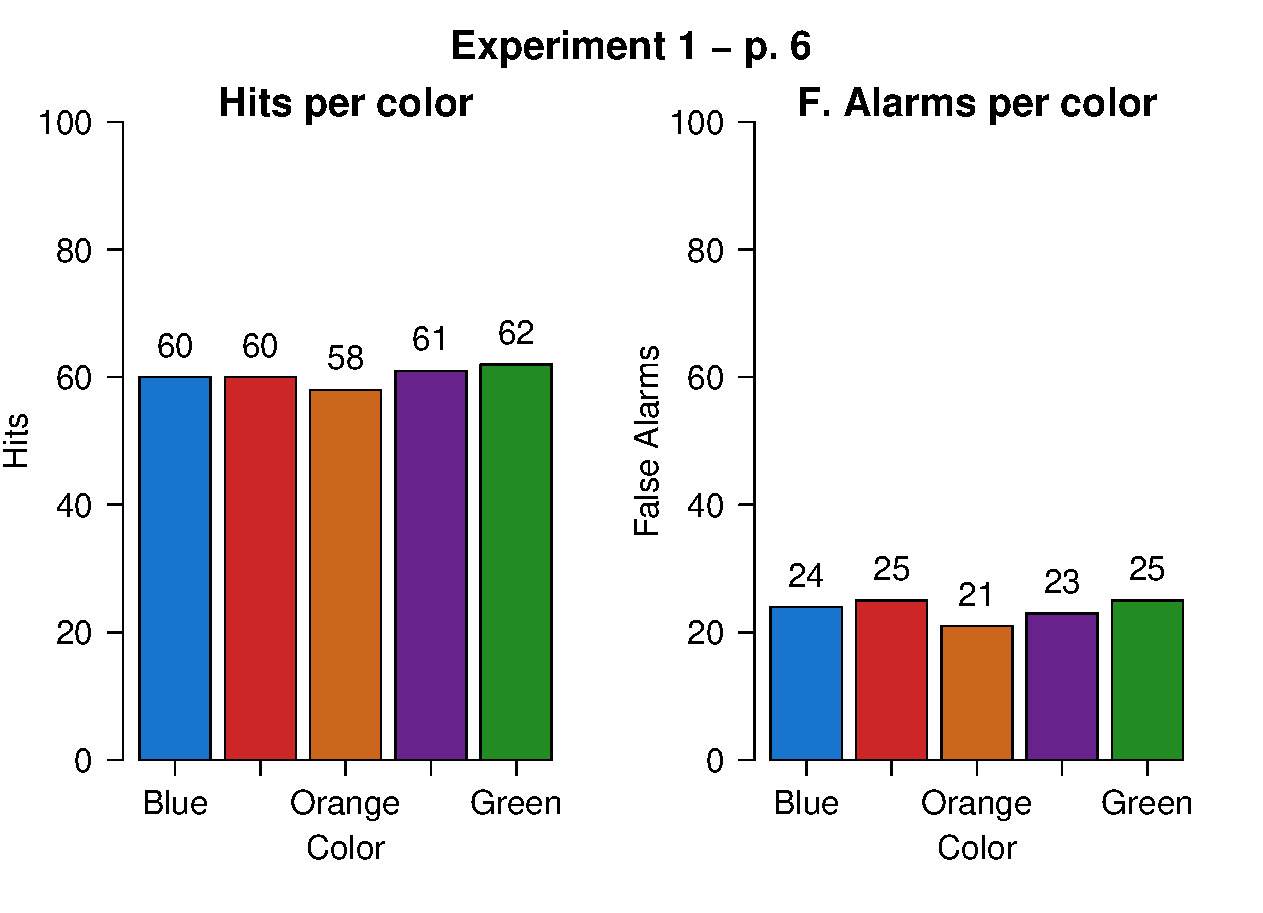
\includegraphics[width=0.45\linewidth]{Figures/8_Color.pdf}
\end{tabular}
\end{center}



\end{itemize}
\end{alertblock}






\end{column} % End of column 2.1
%----------------------------------------------------------------------------------------

%----------------------------------------------------------------------------------------
%   BAYESIAN MODELING 
%----------------------------------------------------------------------------------------
\setlength{\onecolwid}{0.21\paperwidth}
\begin{column}{\sepwid}\end{column} % Empty spacer column
\begin{column}{\onecolwid}\vspace{-2.1in} % The second column within column 2 (column 2.2)


%Agregamos un espacio para que la columna 2.2 no se encime con el Spoiler
\setbeamercolor{item}{fg=white}
\setbeamercolor{item projected}{fg=white,bg=white}
\begin{itemize}
\item
\item
\end{itemize}



\setbeamercolor{block alerted title}{fg=white,bg=jblue} % Change the alert block title colors
\setbeamercolor{block alerted body}{fg=black,bg=white} % Change the alert block body colors
\begin{alertblock}{Bayesian Modeling}


% set colors for itemize/enumerate
\setbeamercolor{item}{fg=Violet}
\setbeamercolor{item projected}{fg=white,bg=Violet}
\begin{enumerate}
\item D' differences: Are conditions actually different?
\begin{center}
\begin{tabular}{ccc}
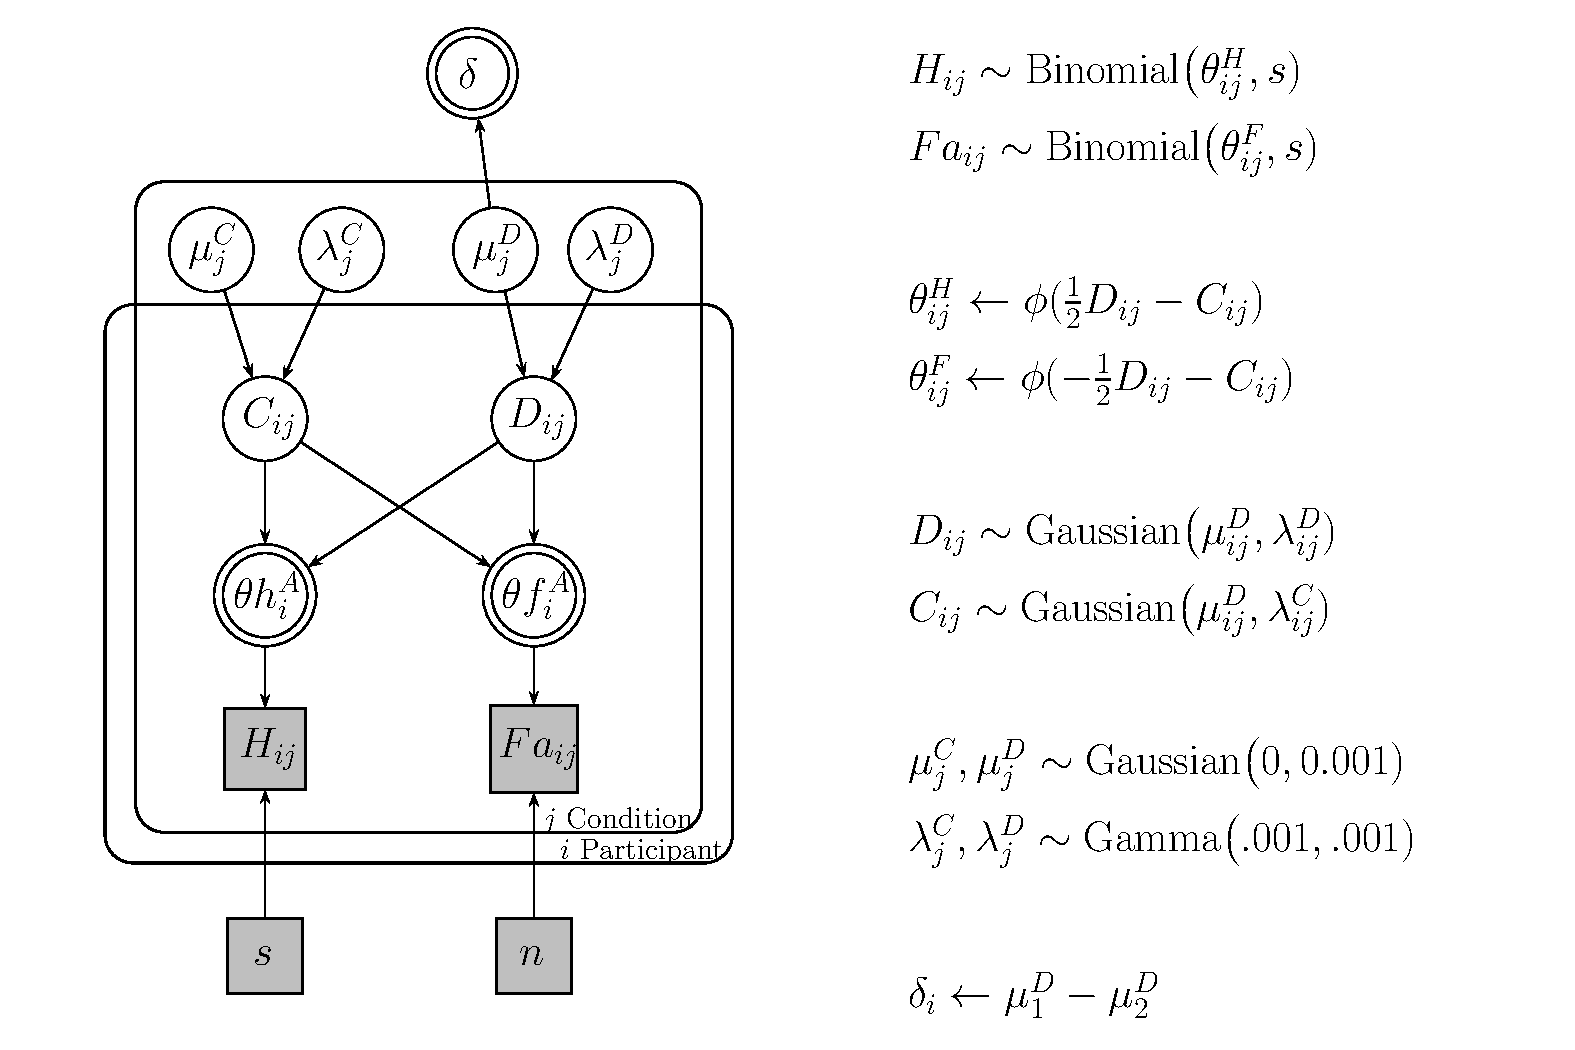
\includegraphics[width=0.65\linewidth]{Figures/Delta_DiffD_Model4.pdf}
\end{tabular}
\end{center}

\begin{center}
\begin{tabular}{ccc}
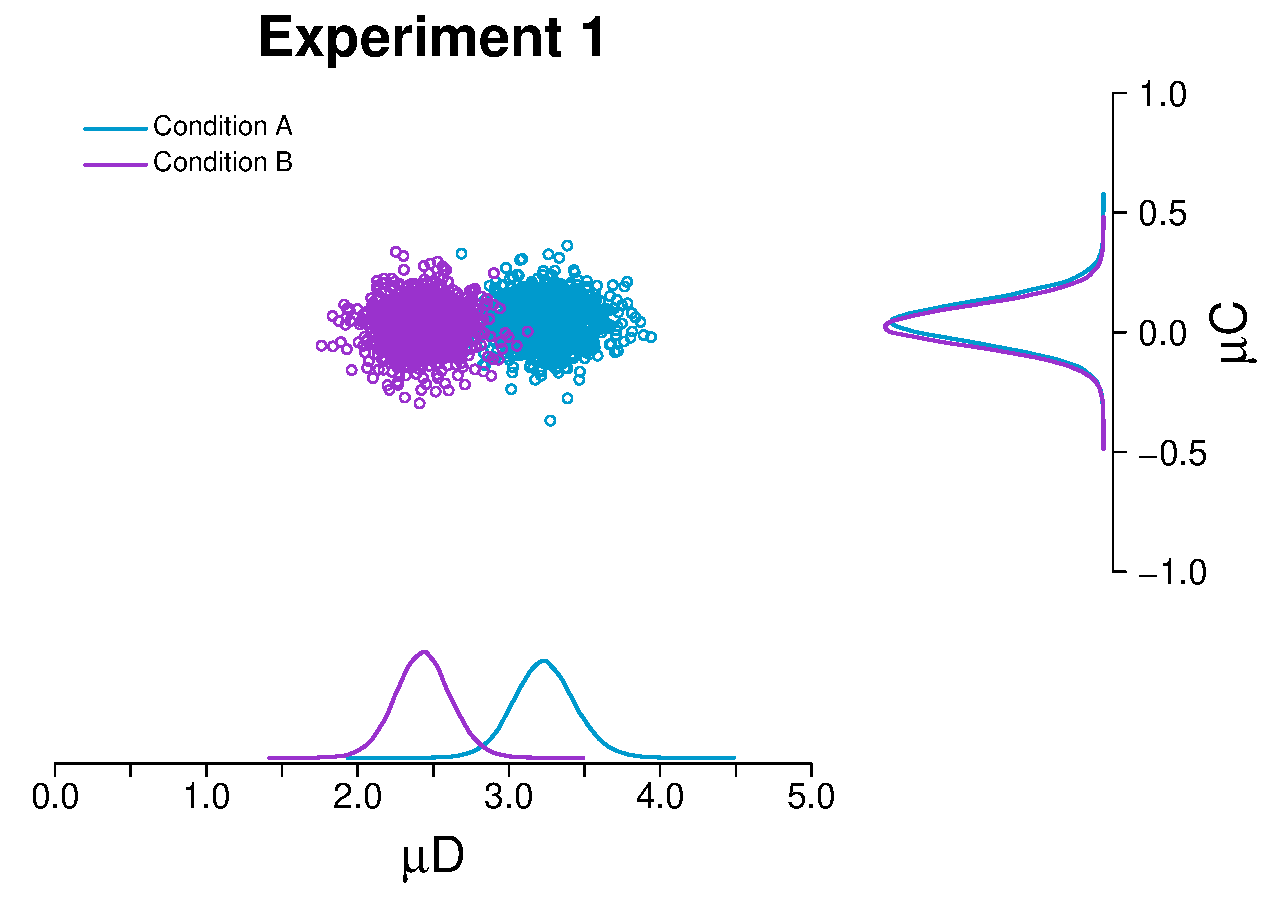
\includegraphics[width=0.45\linewidth]{Figures/Modelo_Delta_MeanDC_1.pdf} & \hfill & 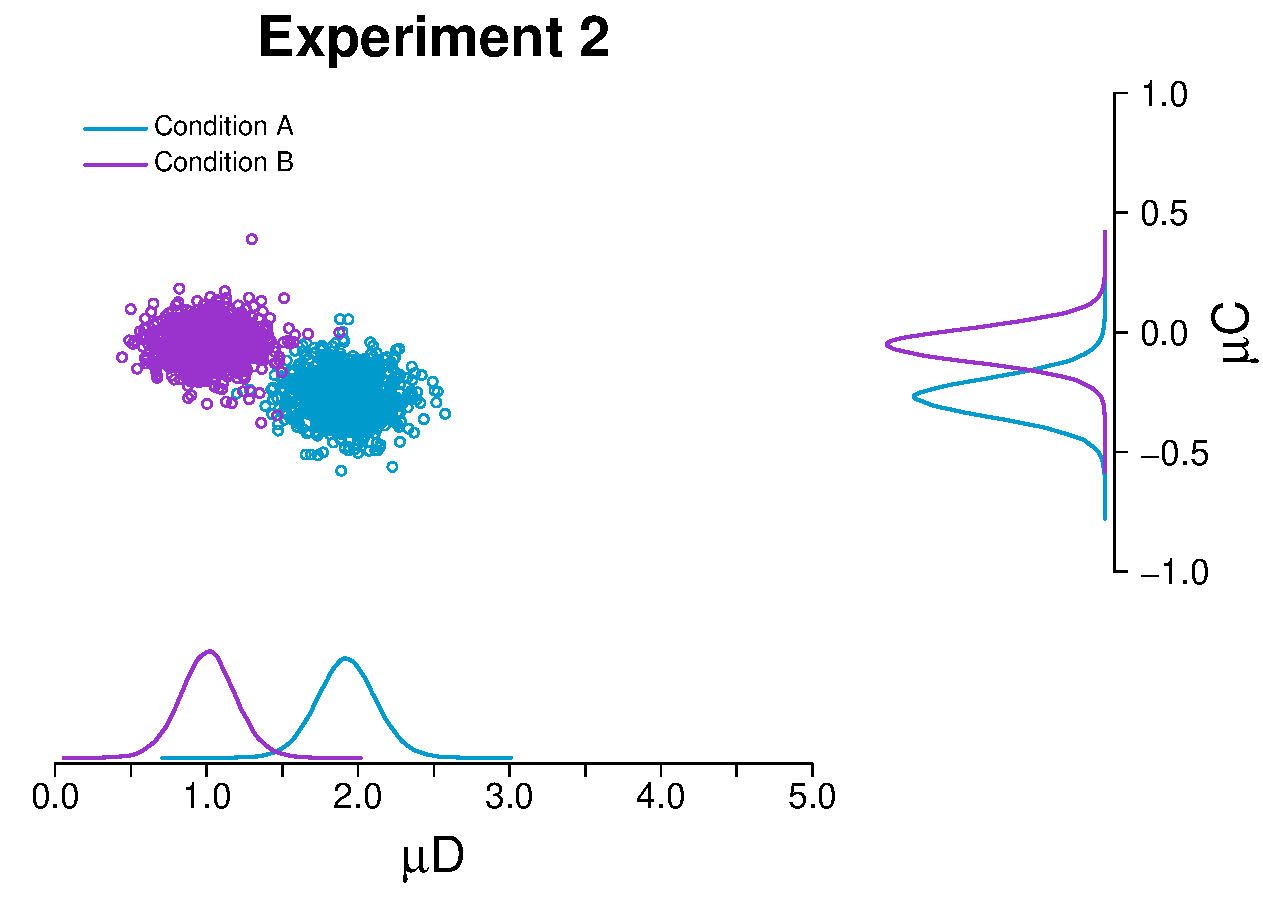
\includegraphics[width=0.45\linewidth]{Figures/Modelo_Delta_MeanDC_2.pdf}
\end{tabular}
\end{center}

\begin{center}
\begin{tabular}{ccc}
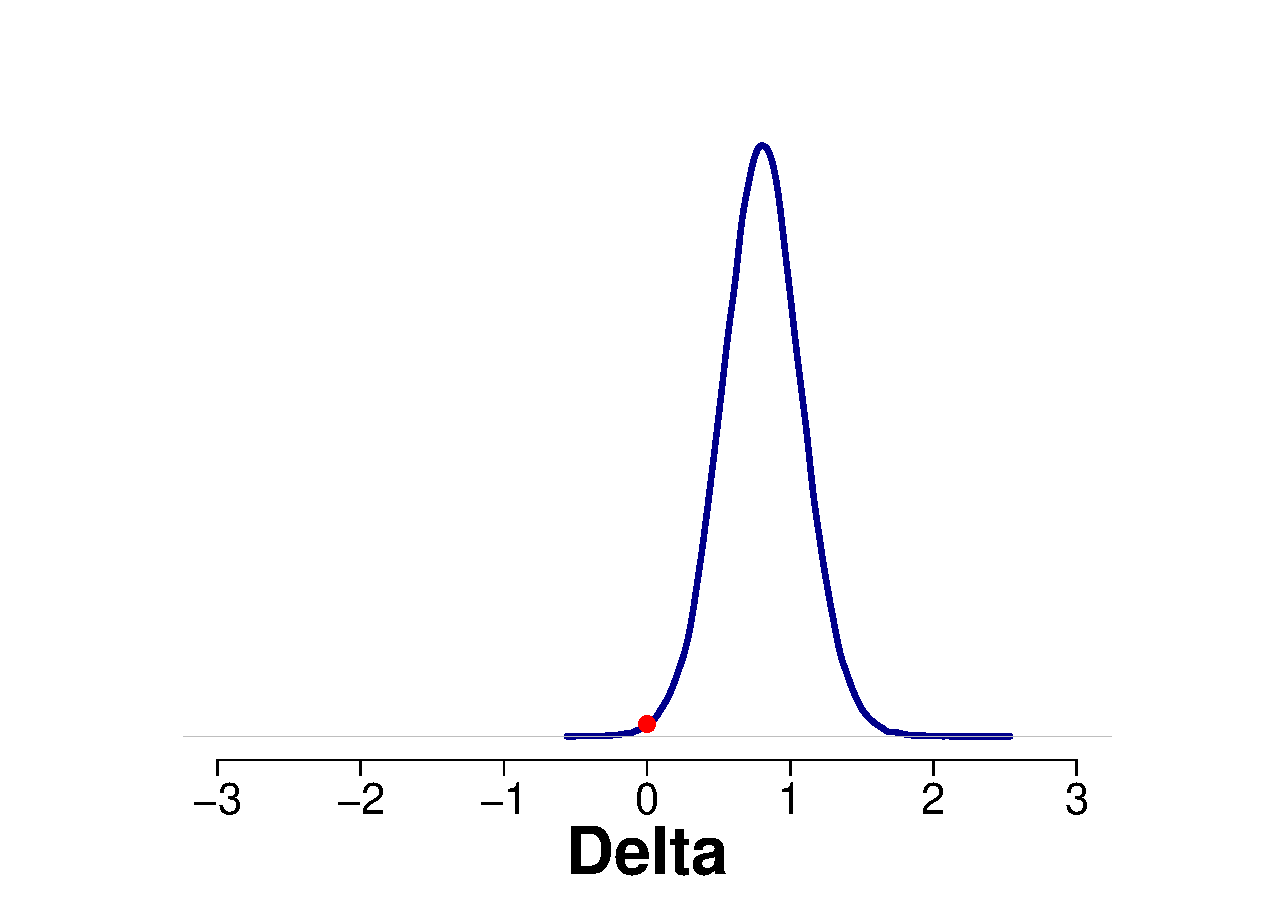
\includegraphics[width=0.35\linewidth]{Figures/Delta_1.pdf}  $\qquad$ $\qquad$ & \hfill & 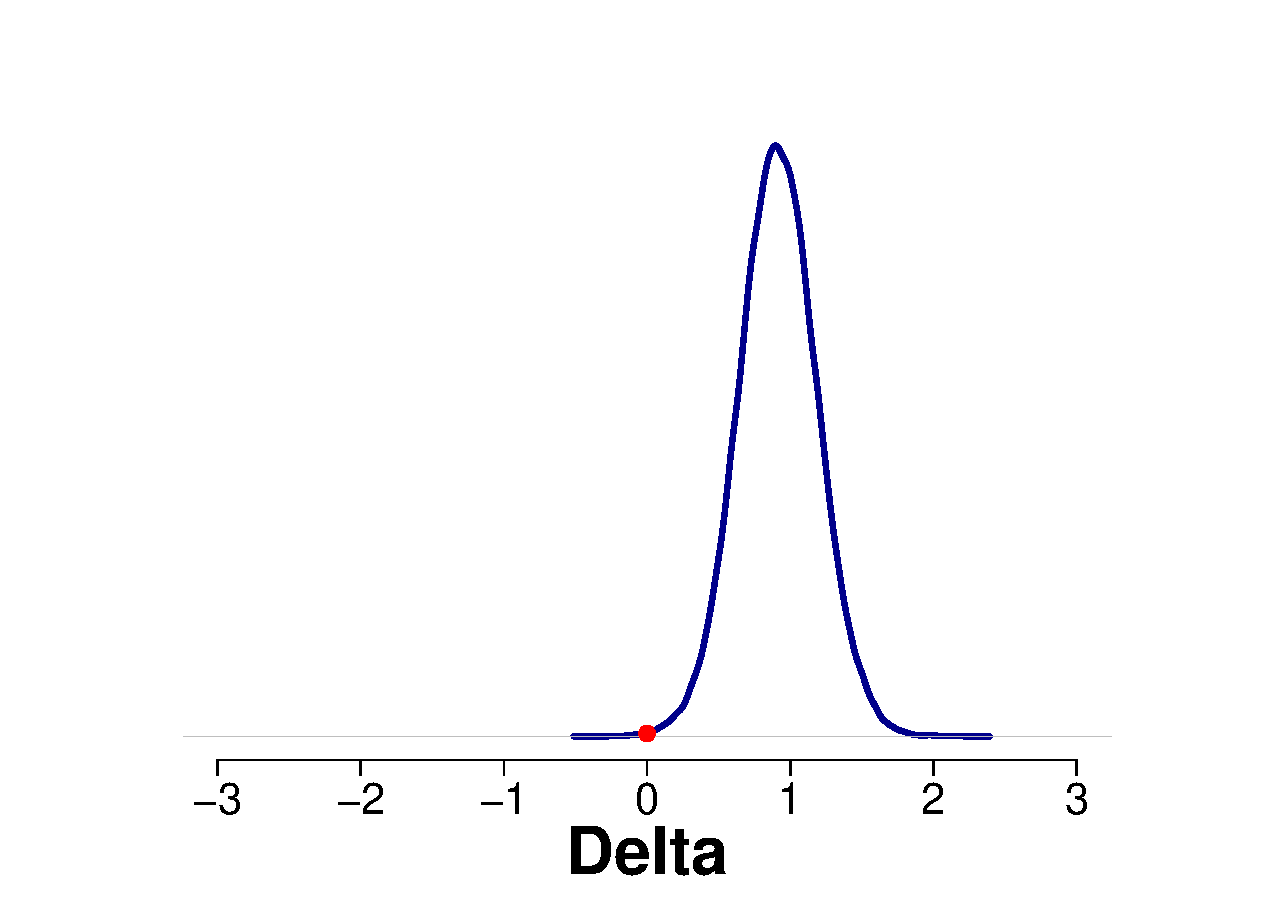
\includegraphics[width=0.35\linewidth]{Figures/Delta_2.pdf}
\end{tabular}
\end{center}



$\qquad$


\item Hit and False Alarm Rate Differences
\begin{center}
\begin{tabular}{ccc}
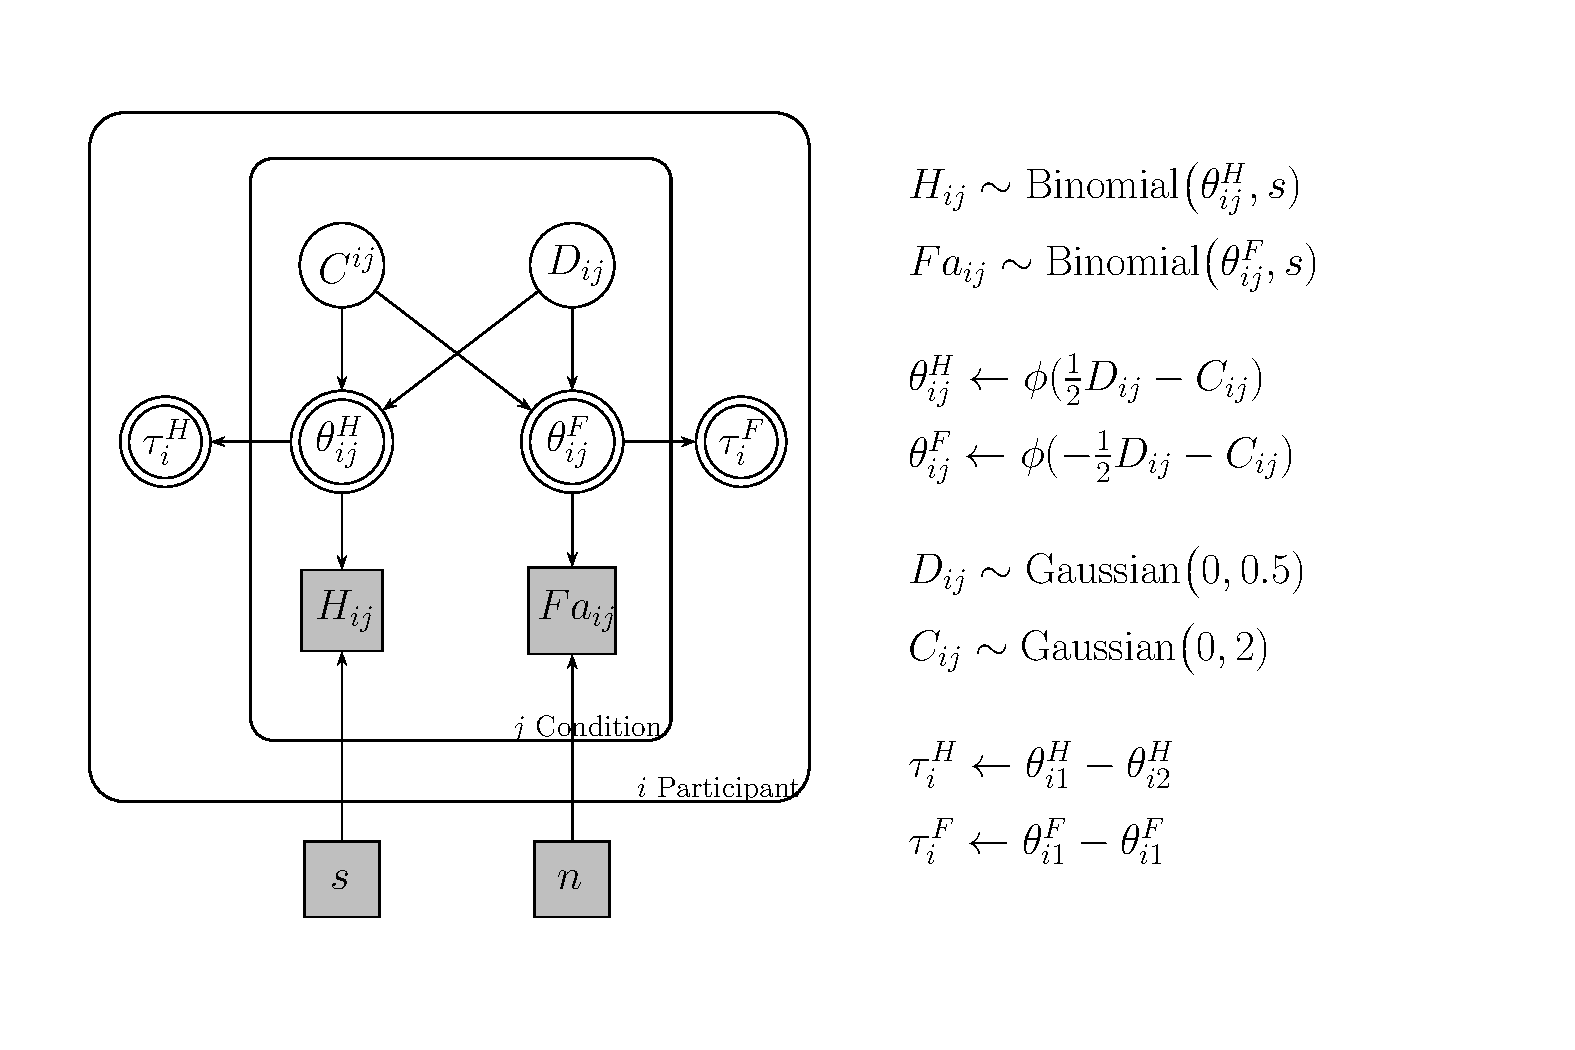
\includegraphics[width=0.65\linewidth]{Figures/Tau_DiffTeta_Model3.pdf}
\end{tabular}


\begin{tabular}{ccc}
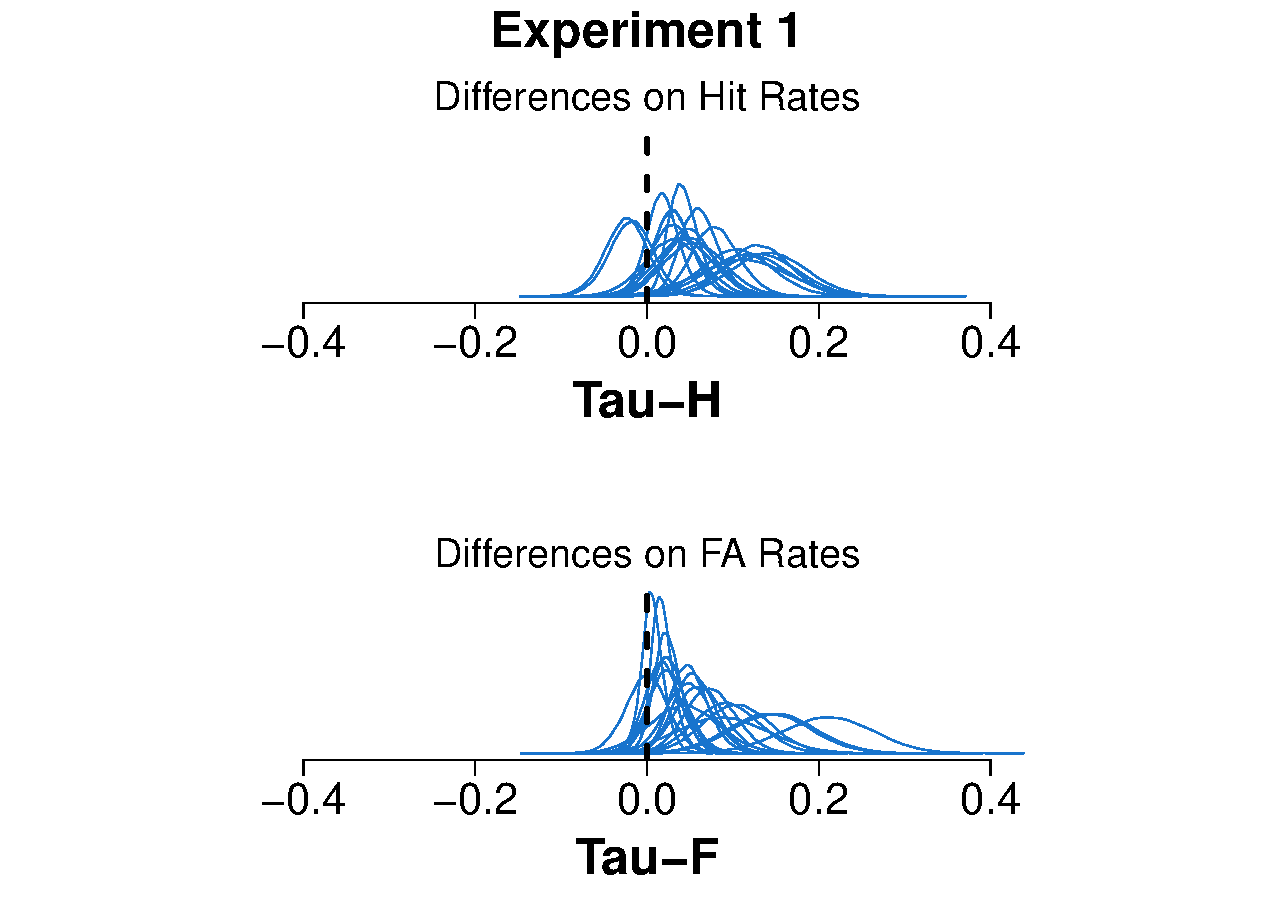
\includegraphics[width=0.48\linewidth]{Figures/Tau_1.pdf} & \hfill & 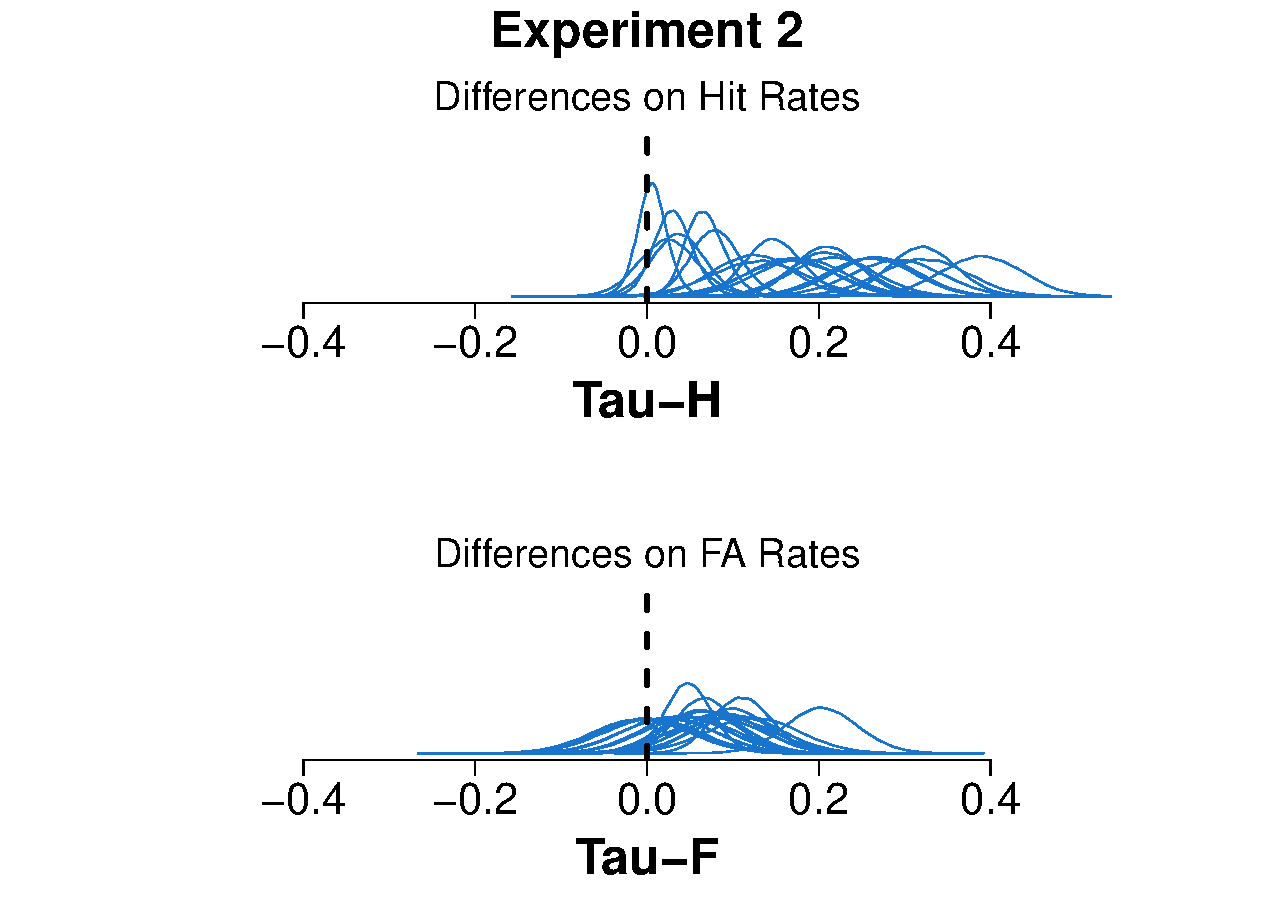
\includegraphics[width=0.48\linewidth]{Figures/Tau_2.pdf}
\end{tabular}
\end{center}



$\quad$
\end{enumerate}
%Lorem ipsum dolor \textbf{sit amet}, consectetur adipiscing elit. Sed laoreet accumsan mattis. Integer sapien tellus, auctor ac blandit eget, sollicitudin vitae lorem. Praesent dictum tempor pulvinar. Suspendisse potenti. Sed tincidunt varius ipsum, et porta nulla suscipit et. Etiam congue bibendum felis, ac dictum augue cursus a. \textbf{Donec} magna eros, iaculis sit amet placerat quis, laoreet id est. In ut orci purus, interdum ornare nibh. Pellentesque pulvinar, nibh ac malesuada accumsan, urna nunc convallis tortor, ac vehicula nulla tellus eget nulla. Nullam lectus tortor, \textit{consequat tempor hendrerit} quis, vestibulum in diam. Maecenas sed diam augue.

\end{alertblock}


\setbeamercolor{block title}{fg=red,bg=white} % Change the block title color

\setbeamercolor{item}{fg=white}
\setbeamercolor{item projected}{fg=white,bg=white}
\setbeamercolor{block title}{fg=jblue,bg=white}
\setbeamercolor{block body}{fg=black,bg=white}
\begin{block}{Acknowledgments \& Contact Information}

\small{\rmfamily{This project was supported by PAPIIT IN307214 and PAPIME PE310016.}} \\

\begin{itemize}
\item Web: \href{https://sites.google.com/site/adaptabilidad25/}{https://sites.google.com/site/adaptabilidad25/}
\item Email: \href{mailto:adrifelcha@gmail.com}{adrifelcha@gmail.com}
\end{itemize}


\end{block}


%\begin{itemize}
%\item
%\end{itemize}


%----------------------------------------------------------------------------------------

\end{column} % End of column 2.2

\end{columns} % End of the split of column 2 - any content after this will now take up 2 columns width

%----------------------------------------------------------------------------------------

\begin{columns}[t,totalwidth=\twocolwid] % Split up the two columns wide column again

\begin{column}{\onecolwid} % The first column within column 2 (column 2.1)

%----------------------------------------------------------------------------------------

\end{column} % End of column 2.1

\end{columns} % End of the split of column 2

\end{column} % End of the second column

\begin{column}{\sepwid}\end{column} % Empty spacer column

\setlength{\onecolwid}{0.252\paperwidth} % Width of one column
\begin{column}{\onecolwid} % The third column

%----------------------------------------------------------------------------------------
%   CONCLUSION
%----------------------------------------------------------------------------------------

\setbeamercolor{block alerted title}{fg=white,bg=jblue} % Titulo
\setbeamercolor{block alerted body}{fg=black,bg=white} % Cuerpo
\begin{alertblock}{Classical Analysis}

% set colors for itemize/enumerate
\setbeamercolor{item}{fg=Purple}
\setbeamercolor{item projected}{fg=white,bg=Purple}
\begin{enumerate}
\item D' differences: Are conditions actually different?
\begin{center}
\begin{tabular}{ccc}
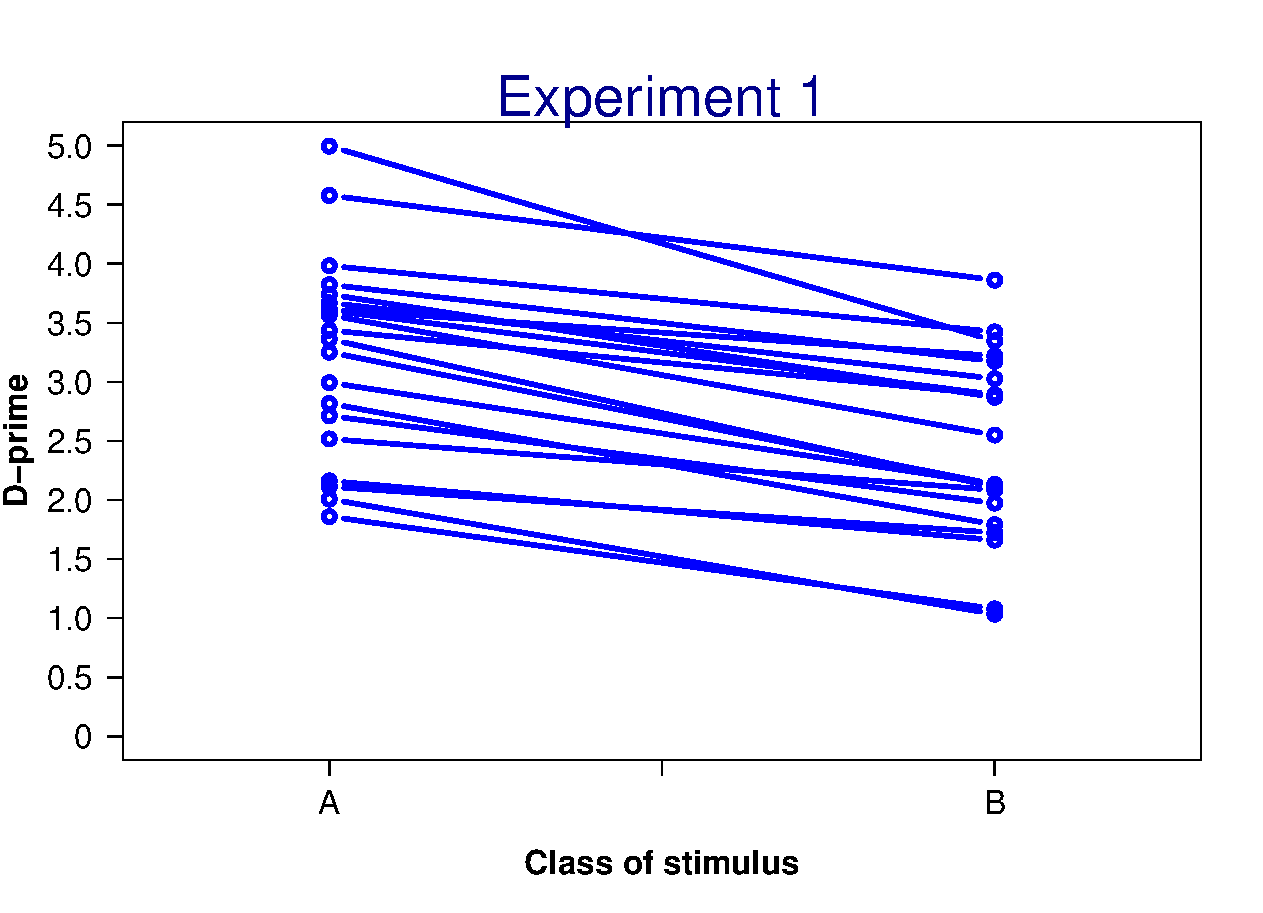
\includegraphics[width=0.45\linewidth]{Figures/An_Diff_D_1.pdf} & \hfill & 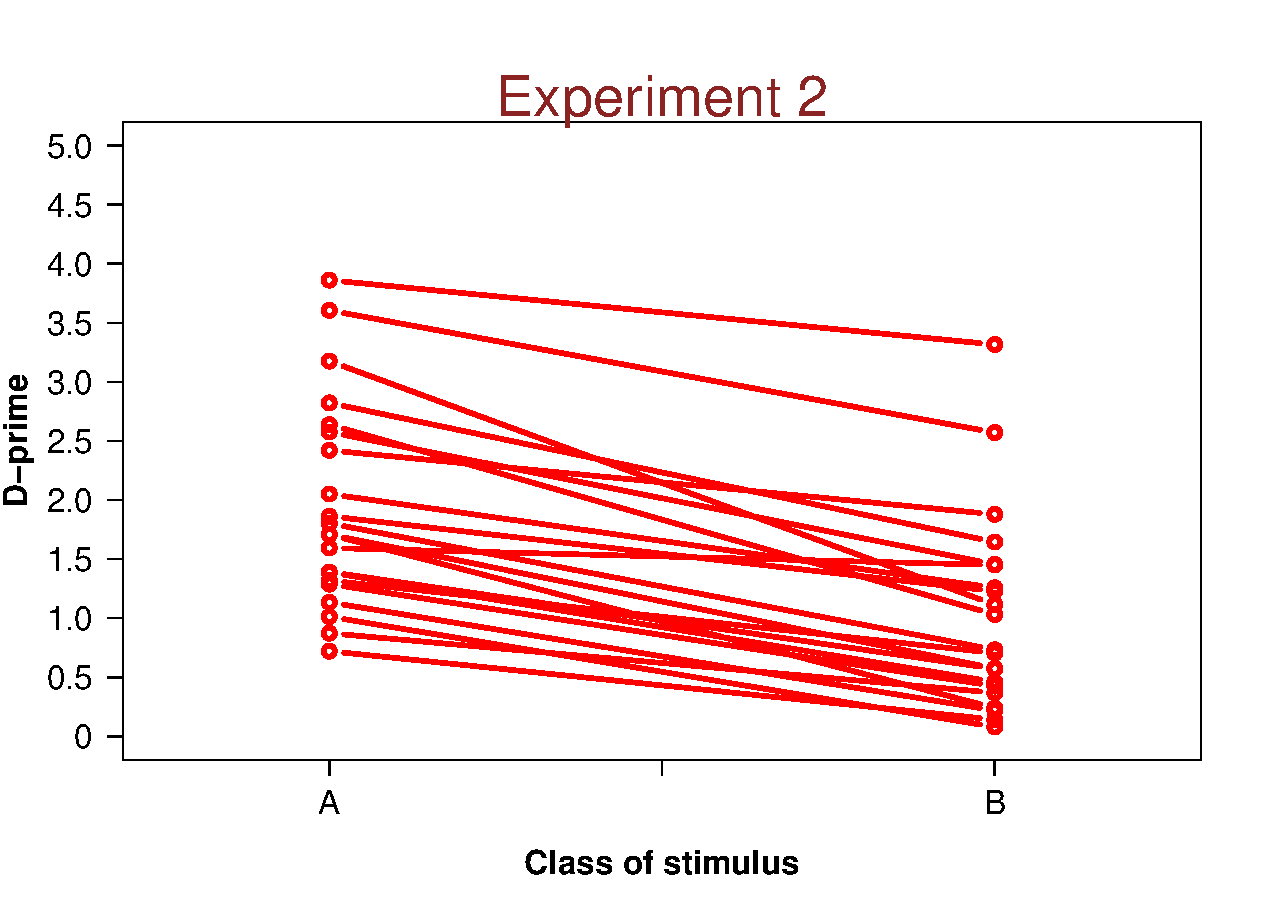
\includegraphics[width=0.45\linewidth]{Figures/An_Diff_D_2.pdf}
\end{tabular}
\end{center}
\begin{table}
\vspace{2ex}
\begin{tabular}{l | c c c c}
\toprule
\textbf{T-test} & \textbf{$\mu$ A} & \textbf{$\mu$ B} & \textbf{T}  & \textbf{P value}\\
\midrule
Experiment 1 & 3.240 & 2.448 & -3.0587 & 0.0020 \\
Experiment 2 & 1.950 & 1.022 & -3.4972 & 0.0005 \\
\bottomrule
\end{tabular}
\end{table}

$\qquad$


\item Differences across Hit and False Alarm Rates
\begin{table}
\vspace{3ex}
\begin{tabular}{l l | c c c c}
\toprule
\textbf{T-test} & \textbf{} & \textbf{$\mu$ A} & \textbf{$\mu$ B} & \textbf{T} & \textbf{P value}\\
\midrule
Exp 1 & Hits & 0.922 & 0.860 & -2.4348 & 0.0098 \\
Exp 1 & FA & 0.08 & 0.143 & 1.917 & 0.0314 \\
Exp 2 & Hits & 0.853 & 0.678 & -3.4757, & 0.0006 \\
Exp 2 & FA & 0.268 & 0.336 & 1.769 & 0.0425 \\
\bottomrule
\end{tabular}
\end{table}

$\quad$

\item Mean Confidence Rating per class of stimuli
\begin{table}
\vspace{3ex}
\begin{tabular}{l l |  c c c c}
\toprule
\textbf{T-test} & \textbf{} & \textbf{$\mu$ A} & \textbf{$\mu$ B} & \textbf{T} & \textbf{P value}\\
\midrule
Exp 1 & Signal & 5.445 & 5.212 & -1.7778, & 0.0418 \\
Exp 1 & Noise & 1.542 & 1.883 & -1.7208 & 0.0472 \\
Exp 2 & Signal & 5.183 & 4.342  & -3.6752, & 0.0004 \\
Exp 2 & Noise & 2.386 & 2.752 & -1.809 & 0.0391 \\
\bottomrule
\end{tabular}
\end{table}
\end{enumerate}
\setbeamercolor{item}{fg=white}
\setbeamercolor{item projected}{fg=white,bg=white}
\begin{itemize}
\item
\end{itemize}
.$\qquad$$\qquad$$\qquad$$\qquad$$\qquad$$\qquad$$\qquad$$\qquad$$\qquad$$\qquad$ Glanzer \& Adams, (1990)
\end{alertblock}



\setbeamercolor{block alerted title}{fg=white,bg=jblue}
\setbeamercolor{block alerted body}{fg=black,bg=jblue!10}
%\setbeamercolor{block alerted title}{fg=white,bg=CadetBlue} % Change the alert block title colors
%\setbeamercolor{block alerted body}{fg=black,bg=white} % Change the alert block body colors
\begin{alertblock}{Discussion}

The present study is the first to show evidence of the Mirror Effect patterns of response on a SD task that does not involve recognition memory. 
\setbeamercolor{item}{fg=white}
\setbeamercolor{item projected}{fg=white,bg=white}
\begin{itemize}
\item
\end{itemize}
The perceptual task here presented lacked a pre-experimental phase where participants had the chance to manipulate how powerful were the illusions elicited in each condition. This suggests that there might be a much more basic principle regulating the Mirror Effect pattern of responses.

\end{alertblock}

%----------------------------------------------------------------------------------------
%   REFERENCES
%----------------------------------------------------------------------------------------

\setbeamercolor{item}{fg=white}
\setbeamercolor{item projected}{fg=white,bg=white}
\setbeamercolor{block alerted title}{fg=white,bg=jblue}
\setbeamercolor{block alerted body}{fg=black,bg=jblue!10}
\begin{alertblock}{References}

\setbeamercolor{item}{fg=WildStrawberry}
\setbeamercolor{item projected}{fg=white,bg=WildStrawberry}
\begin{itemize}
\item Glanzer, M., Adams, J. (1990) The Mirror Effect in Recognition Memory \: Data and Theory.\textit{Journal of Experimental Psychology: Learning, Memory and Cognition, 16} (1), 5-16.
\item Glanzer, M., Adams, J., Iverson, G. \& Kim, K. (1993) The Regularities of Recognition Memory. \textit{Psychological Review, 100} (3), 546-567.
\item Massaro, D., Anderson, N. (1971). Judgmental model of the Ebbinghaus Illusion. \textit{Journal of Experimental Psychology, 89}, 147 - 151.
\end{itemize}

%\nocite{*} % Insert publications even if they are not cited in the poster
%\small{\bibliographystyle{unsrt}
%\bibliography{sample}\vspace{0.75in}}

\end{alertblock}

%----------------------------------------------------------------------------------------
%   ACKNOWLEDGEMENTS
%----------------------------------------------------------------------------------------



\end{column} % End of the third column
\end{columns} % End of all the columns in the poster
\end{frame} % End of the enclosing frame
\end{document}

              